% Decision guide for choosing a validation design (based on the meta-analysis results)
\documentclass[border=4pt]{standalone}
\usepackage[T1]{fontenc}
\usepackage[scaled]{helvet}
\renewcommand{\familydefault}{\sfdefault}
\usepackage{tikz}
\usetikzlibrary{positioning,arrows.meta,shapes.geometric}
\definecolor{q}{HTML}{DCEAF7}\definecolor{ql}{HTML}{0072B2}
\definecolor{rnd}{HTML}{E8E8E8}\definecolor{sp}{HTML}{F6DCEB}\definecolor{spl}{HTML}{CC79A7}
\definecolor{ind}{HTML}{FBE3D6}\definecolor{indl}{HTML}{D55E00}
\begin{document}
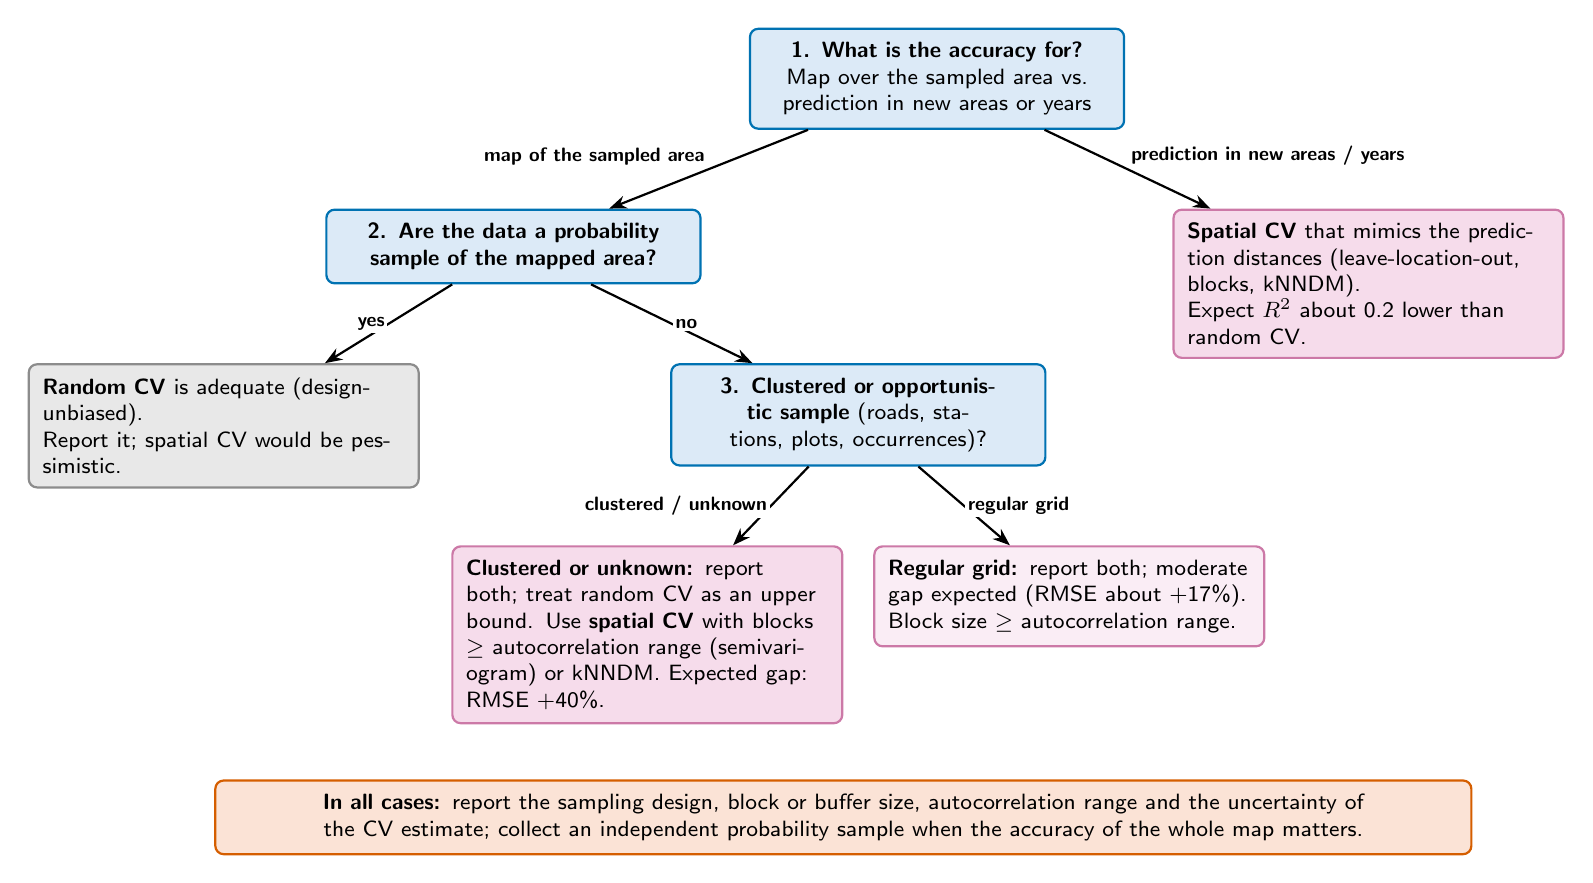
\begin{tikzpicture}[font=\footnotesize,
  qn/.style={draw=ql, fill=q, rounded corners=3pt, thick, align=center, text width=4.4cm, inner sep=5pt},
  an/.style={rounded corners=3pt, thick, align=left, text width=4.6cm, inner sep=5pt},
  ar/.style={-{Stealth[length=2.2mm]}, thick},
  lab/.style={font=\scriptsize\bfseries, fill=white, inner sep=1pt}]

\node[qn] (q1) {\textbf{1. What is the accuracy for?}\\Map over the sampled area vs.\ prediction in new areas or years};
\node[qn, below left=1.0cm and 0.6cm of q1] (q2) {\textbf{2. Are the data a probability sample of the mapped area?}};
\node[an, draw=spl, fill=sp, below right=1.0cm and 0.6cm of q1] (a1) {\textbf{Spatial CV} that mimics the prediction distances (leave-location-out, blocks, kNNDM).\\Expect $R^2$ about 0.2 lower than random CV.};

\node[an, draw=black!45, fill=rnd, below left=1.0cm and -1.2cm of q2] (a2) {\textbf{Random CV} is adequate (design-unbiased).\\Report it; spatial CV would be pessimistic.};
\node[qn, below right=1.0cm and -0.4cm of q2] (q3) {\textbf{3. Clustered or opportunistic sample} (roads, stations, plots, occurrences)?};

\node[an, draw=spl, fill=sp, below left=1.0cm and -2.2cm of q3] (a3) {\textbf{Clustered or unknown:} report both; treat random CV as an upper bound. Use \textbf{spatial CV} with blocks $\geq$ autocorrelation range (semivariogram) or kNNDM. Expected gap: RMSE +40\%.};
\node[an, draw=spl, fill=sp!50, below right=1.0cm and -2.2cm of q3] (a5) {\textbf{Regular grid:} report both; moderate gap expected (RMSE about +17\%). Block size $\geq$ autocorrelation range.};

\draw[ar] (q1) -- node[lab, above left] {map of the sampled area} (q2);
\draw[ar] (q1) -- node[lab, above right] {prediction in new areas / years} (a1);
\draw[ar] (q2) -- node[lab, left] {yes} (a2);
\draw[ar] (q2) -- node[lab, right] {no} (q3);
\draw[ar] (q3) -- node[lab, left] {clustered / unknown} (a3);
\draw[ar] (q3) -- node[lab, right] {regular grid} (a5);

\node[an, draw=indl, fill=ind, text width=15.6cm, align=center, below=0.7cm of a3.south east, anchor=north] (a4)
  {\textbf{In all cases:} report the sampling design, block or buffer size, autocorrelation range and the uncertainty of the CV estimate; collect an independent probability sample when the accuracy of the whole map matters.};
\end{tikzpicture}
\end{document}
